% ============================================================
%  TASK 4.2 — TWO-DIODE TOPOLOGY WITH MICROSTRIP LINES
% ============================================================

\section{Task 4.2 --- Two-Diode Topology with Microstrip Lines}
\label{sec:task4_2}

This section repeats the microstrip implementation steps from Task 3.2, but here, we are progressively replacing the components of the matching network with microstrip lines. The goal, as explained before, is to move closer to a circuit that can realistically be implemented on a PCB, where the physical routes play an active role in impedance matching. The final goal is to compare the results with those obtained using only LC circuit.

% ------------------------------------------------------------
\subsection{Substrate and design rules}
\label{subsec:2d_design_rules}
% ------------------------------------------------------------

The physical PCB implementation has the exact same design rules as previously established:
%
\begin{itemize}
    \item Substrate: Rogers 4350B ($\varepsilon_r = 4.5$,
          $\tan\delta = 0.02$, $H = \SI{1.6}{\milli\meter}$,
          copper thickness $T = \SI{35}{\micro\meter}$ in ADS model);
    \item Signal traces: characteristic impedance $Z_0 = \SI{50}{\ohm}$,
          corresponding to $W = \SI{3.034}{\milli\meter}$;
    \item Microstrip line length constraints:
          $\SI{3}{\milli\meter} \leq L_\mathrm{line} \leq \SI{10}{\milli\meter}$;
    \item SMD package: 0603.
\end{itemize}

% ------------------------------------------------------------
\subsection{Simplified topology with microstrip re-tuning}
\label{subsec:2d_ms_tuning}
% ------------------------------------------------------------

To reduce design complexity while accounting for the physical traces, a hybrid matching network is implemented. It combines microstrip lines with discrete components. 

\begin{figure}[H]
    \centering
    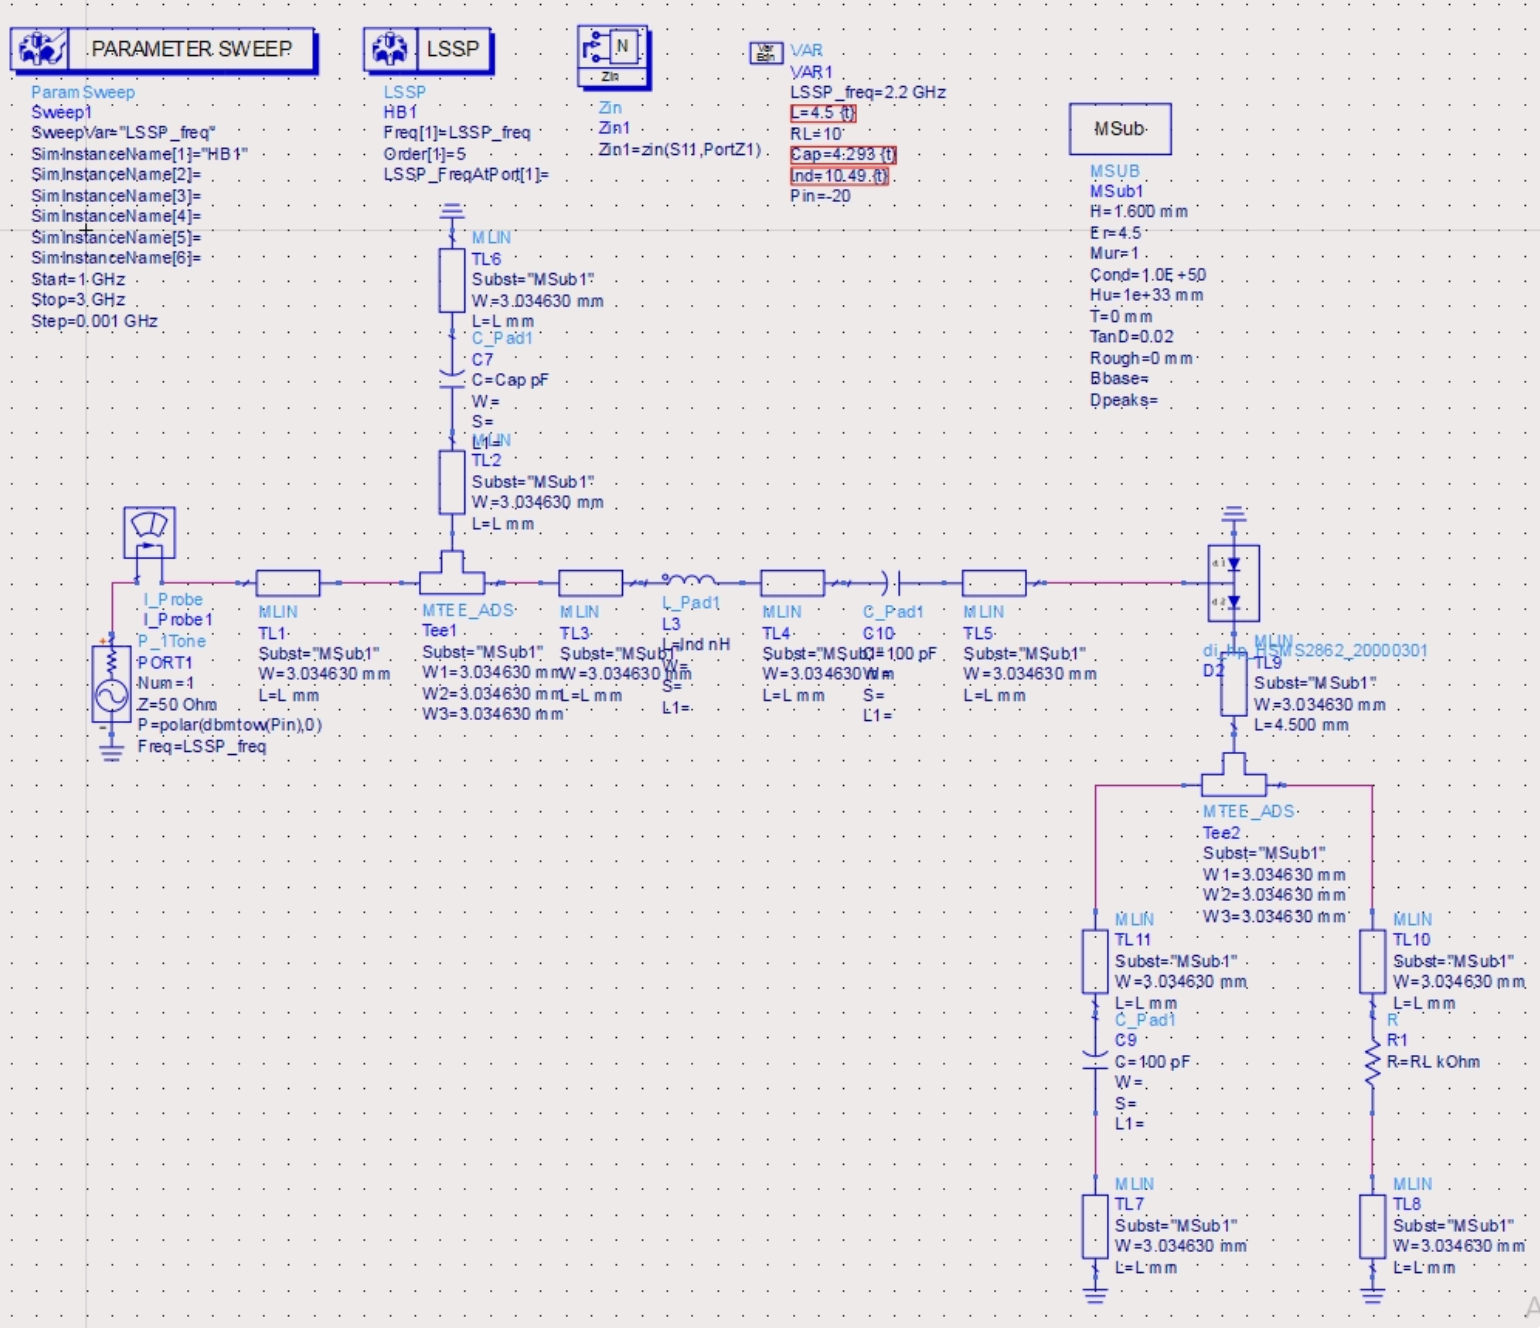
\includegraphics[width=\linewidth]{images/schema_2d_ms.png} 
    \caption{ADS simulation of the two-diode rectifier with inductor, capacitor and microstrip lines matching circuit.}
    \label{fig:schema_2d_ms}
\end{figure}
By using the tune mode of ADS, we managed again to find right parameters and the right $S_{11}$ at our frequency : 
\begin{figure}[H]
    \centering
    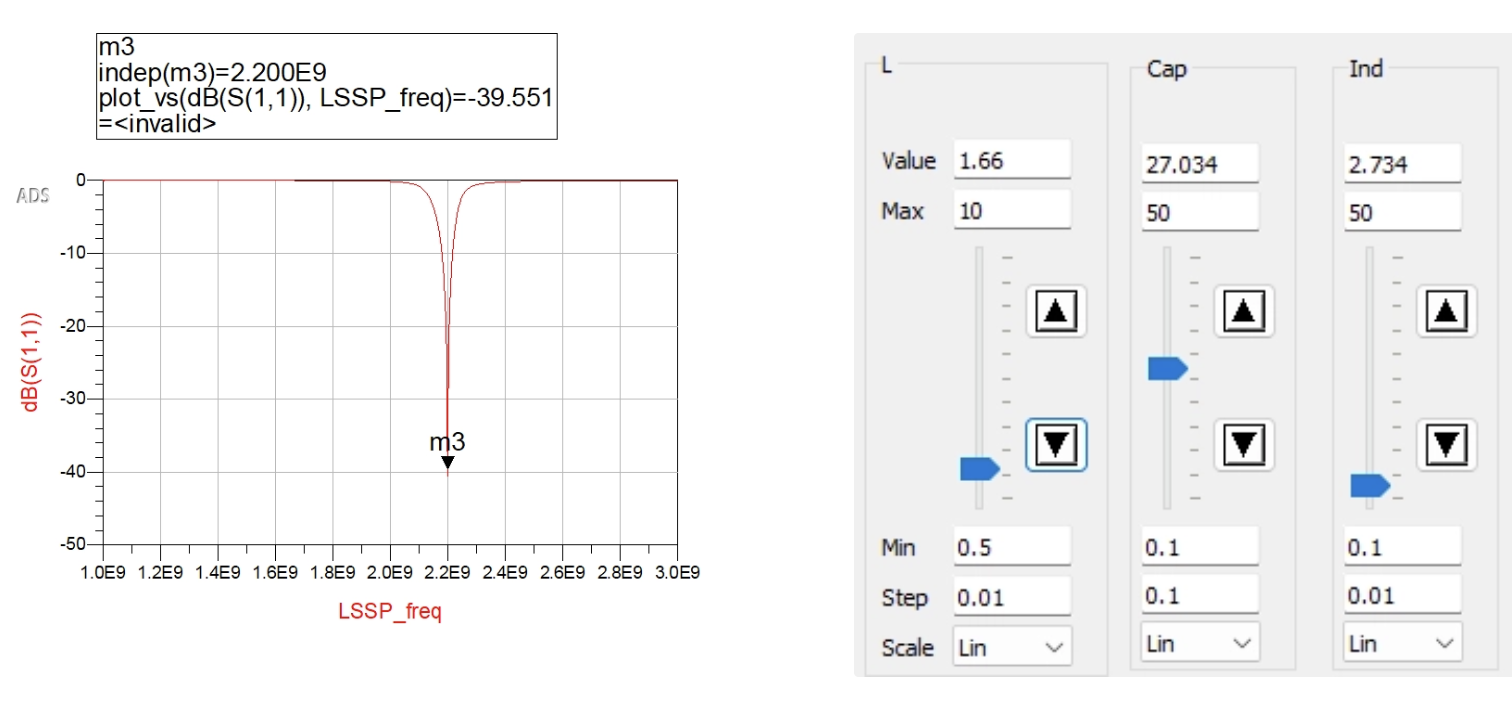
\includegraphics[width=\linewidth]{images/res_2d_ms_simple.png} 
    \caption{ADS results and paramaters of the two-diode rectifier with inductor, capacitor and microstrip lines matching circuit.}
    \label{fig:res_2d_ms_simple}
\end{figure}

% ------------------------------------------------------------
\subsection{Complete microstrip topology re-tuning}
\label{subsec:2d_complete_ms_tuning}
% ------------------------------------------------------------
The introduction of microstrip traces introduces parasitic inductances and capacitances, shifting the resonance frequency. A new parameter sweep in ADS over the microstrip dimensions and the components values determined the optimal tuning. The full set of tuning parameters are listed in Table~\ref{tab:microstrip_2d_tune}.
First, here is the schematic done : 

\begin{figure}[H]
    \centering
    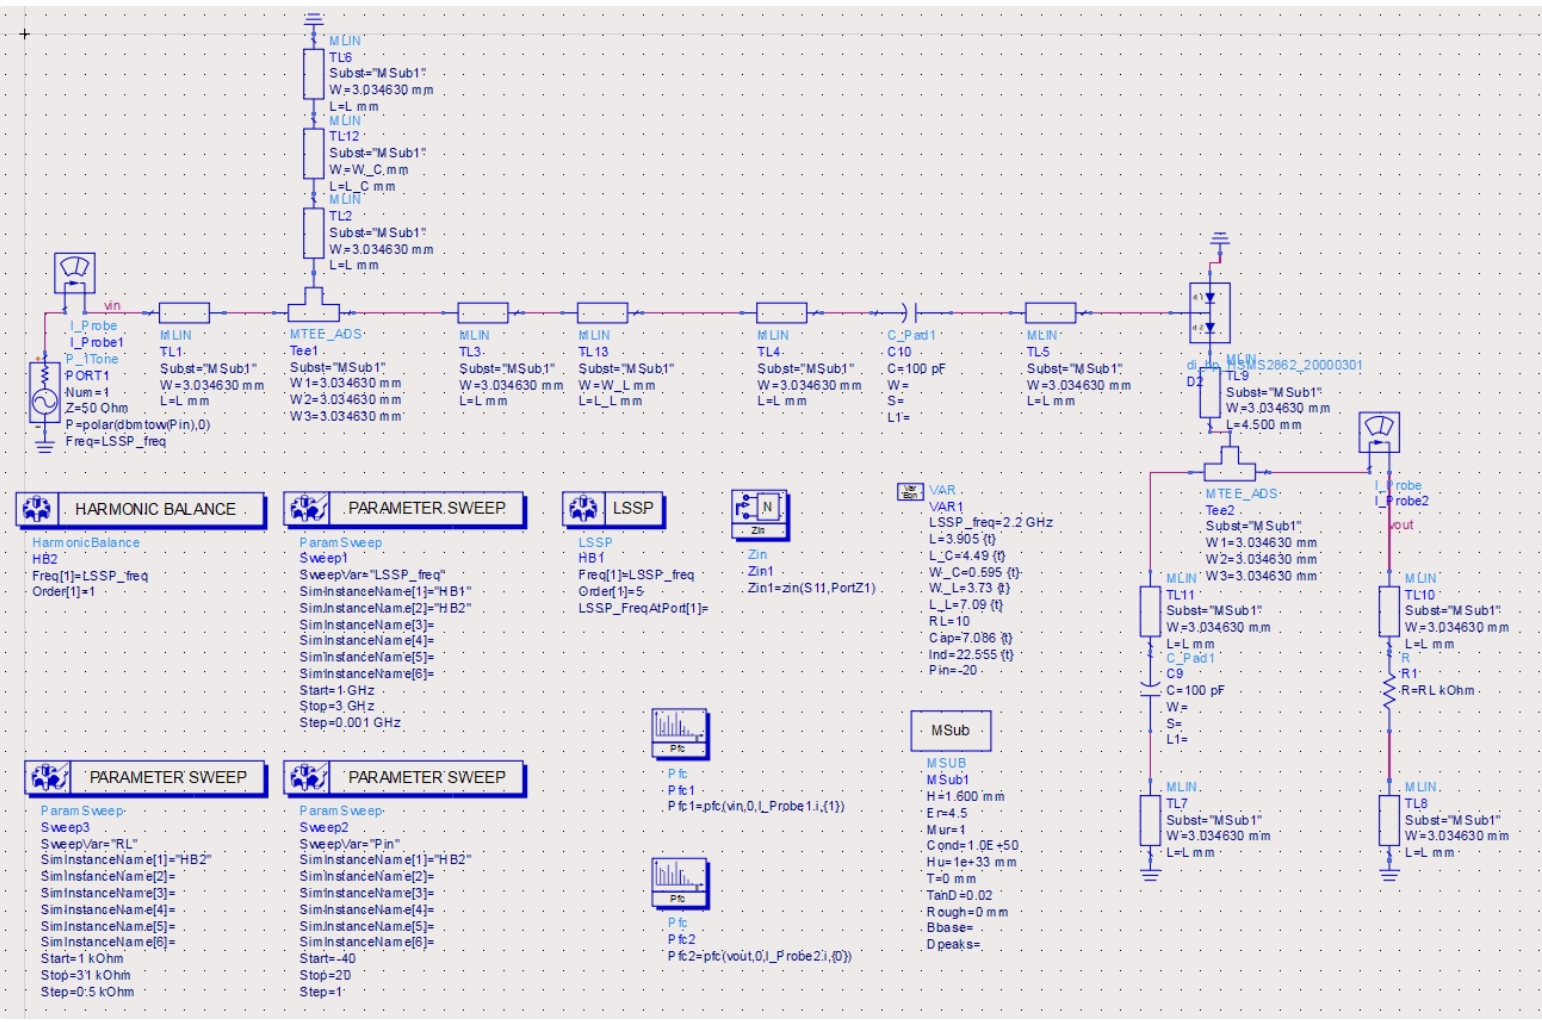
\includegraphics[width=\linewidth]{images/sch_2d_comp_ms.png} 
    \caption{ADS results and paramaters of the two-diode rectifier with inductor, capacitor and microstrip lines matching circuit.}
    \label{fig:sch_2d_comp_ms}
\end{figure}

\begin{table}[H]
    \centering
    \caption{Optimized parameter values for the microstrip matching circuit (two-diode topology, \SI{2.2}{\giga\hertz}).}
    \label{tab:microstrip_2d_tune}
    \begin{tabular}{lll}
        \toprule
        Parameter & Physical meaning & Optimized value \\
        \midrule
        $W_C$ & Width of capacitive stub      & \SI{0.595}{\milli\meter} \\
        $L_C$ & Length of capacitive stub     & \SI{4.49}{\milli\meter} \\
        $W_L$ & Width of inductive stub       & \SI{1.34}{\milli\meter} \\
        $L_L$ & Length of inductive stub      & \SI{8.6}{\milli\meter} \\
        $L$   & Main line segment length      & \SI{3.905}{\milli\meter} \\
        Cap   & Residual lumped capacitance   & \SI{11.1}{\pico\farad} \\
        Ind   & Residual lumped inductance    & \SI{3.9}{\nano\henry} \\
        \bottomrule
    \end{tabular}
\end{table}

The results are shown in Figure~\ref{fig:s11_2d_comp_ms}:
\begin{figure}[H]
    \centering
    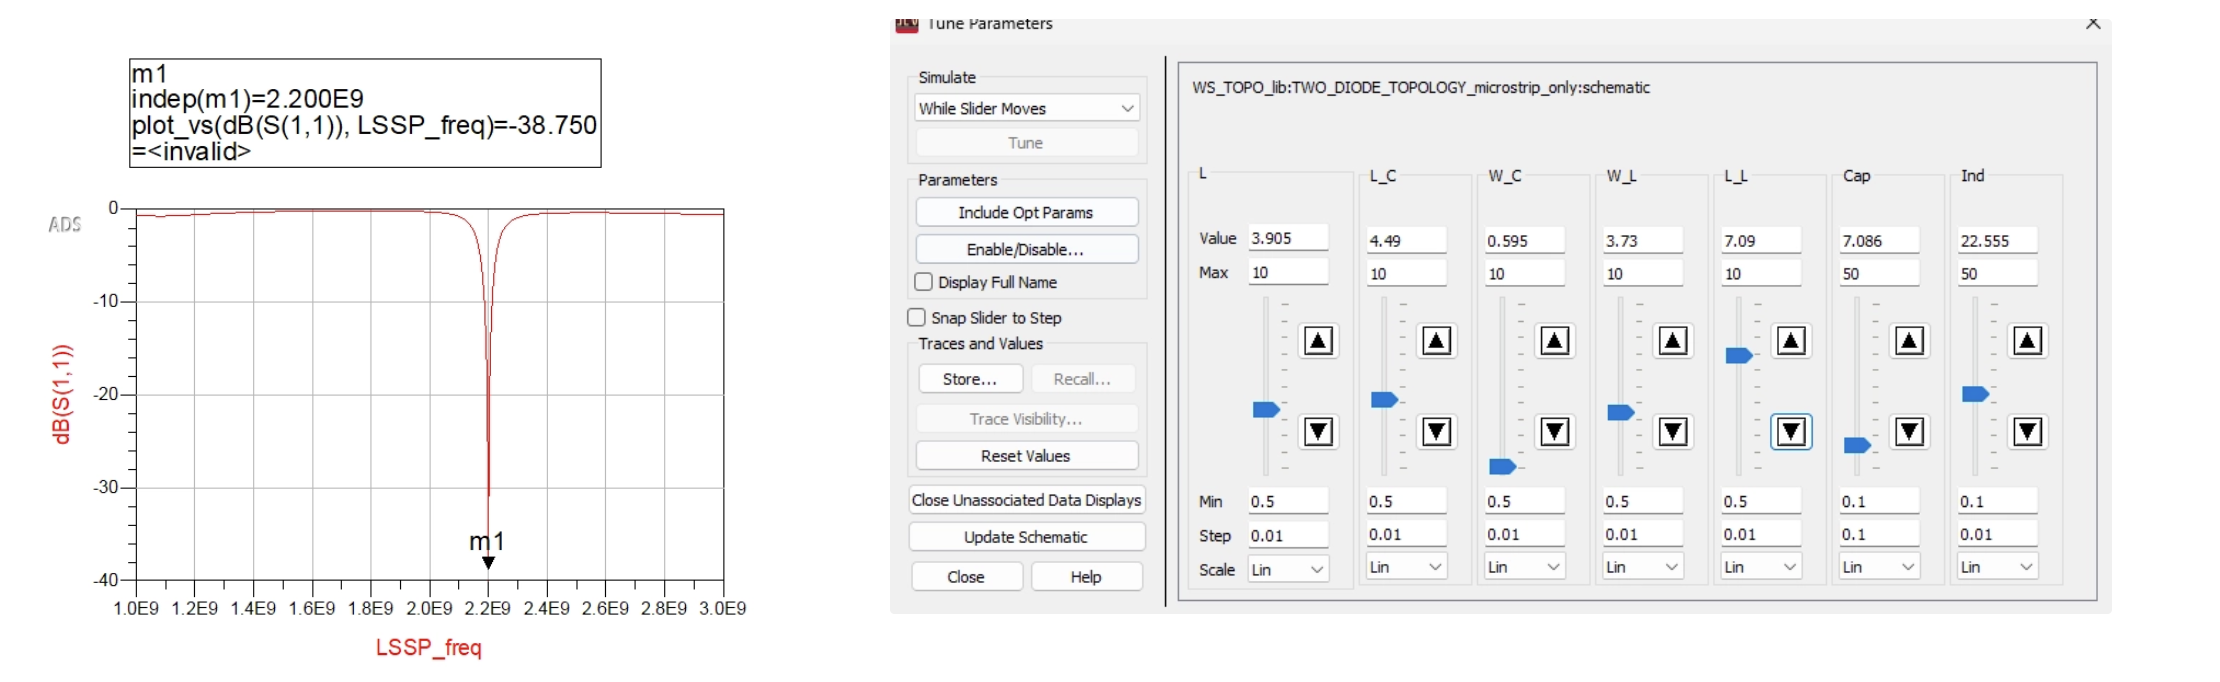
\includegraphics[width=\linewidth]{images/s11_2d_comp_ms.png} % <-- Capture S11 page 31 (-38.749 dB)
    \caption{$S_{11}$ of the matching circuit with only microstrip lines, after parameter sweep re-tuning.}
    \label{fig:s11_2d_comp_ms}
\end{figure}

With these values, the $S_{11}$ reaches an excellent \textbf{\SI{-38.75}{\deci\bel}} at \SI{2.2}{\giga\hertz}, confirming that the topology is perfectly matched after re-tuning.

% ------------------------------------------------------------
\subsection{Rectifier Performance and Topology Comparison}
\label{subsec:2d_performance_comparison}
% ------------------------------------------------------------
Next, we evaluate the full performance of the two-diode voltage doubler
topology under two matching configurations: the LC circuit (Task~4.1) and the pure microstrip circuit (Task~4.2).

% --- Hybrid LC + Microstrip ---
\paragraph{LC Matching Circuit}

Here is the schematic of the hybrid LC + microstrip matching circuit:

\begin{figure}[H]
    \centering
    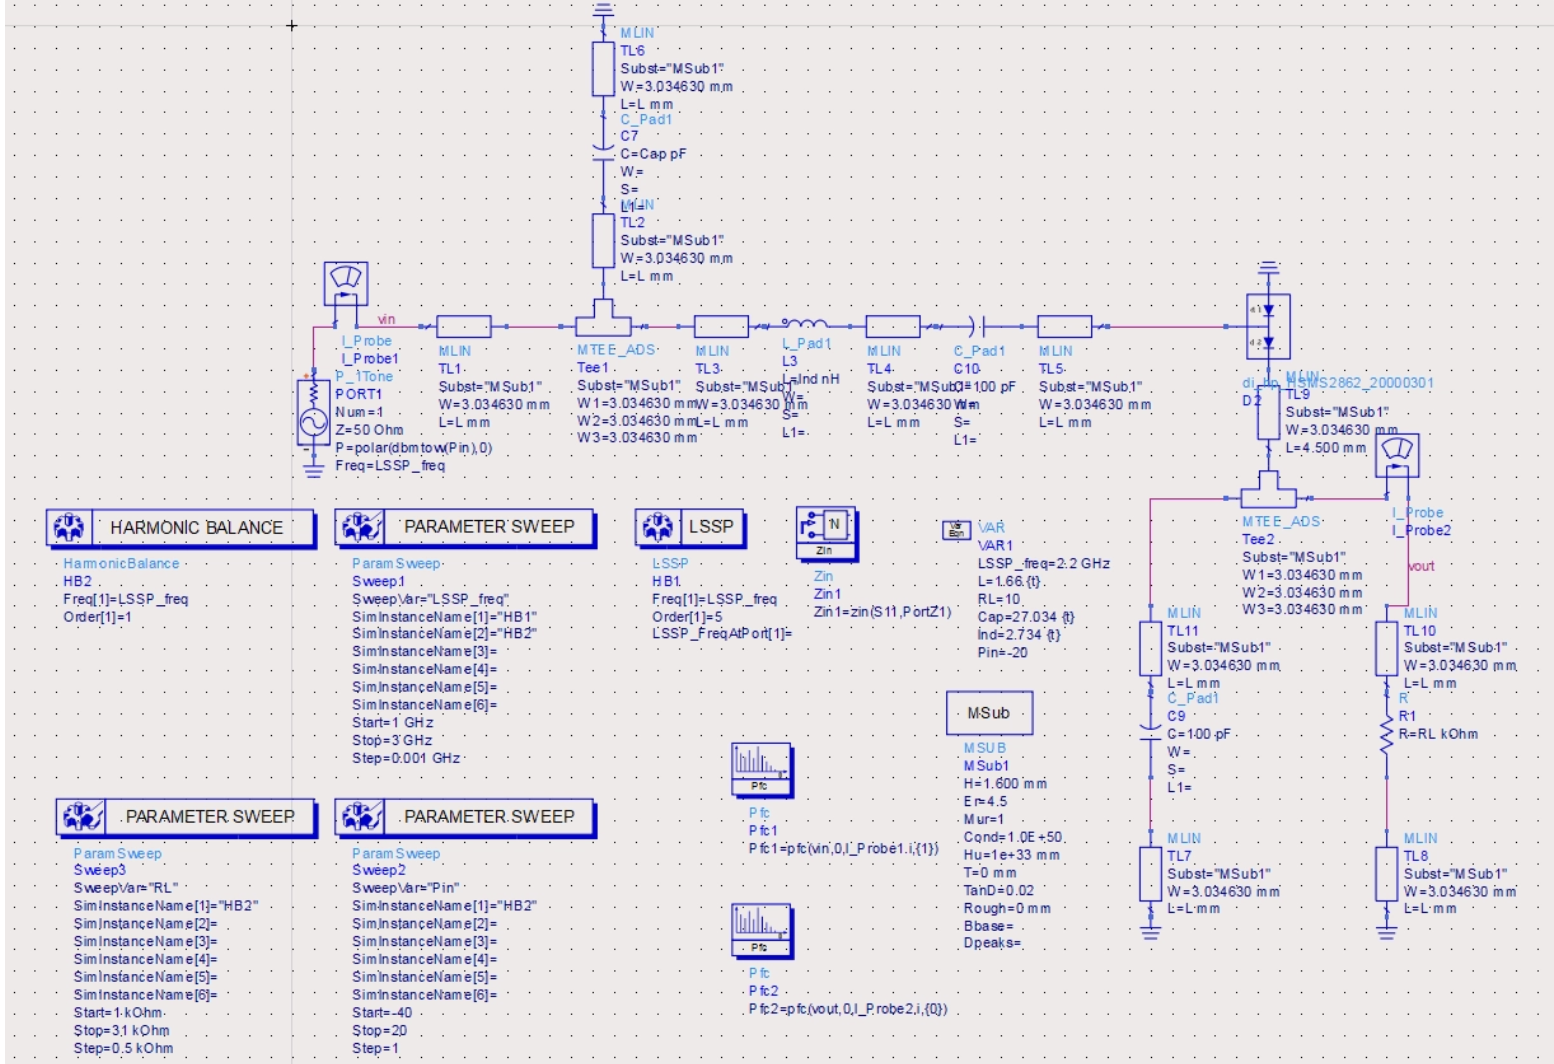
\includegraphics[width=\linewidth]{images/HB_sch_2d_LC_ms.png}
    \caption{Harmonic Balance simulation schematic for the 2-Diode
             topology with LC + microstrip matching
             ($f = \SI{2.2}{\giga\hertz}$, $R_L = \SI{10}{\kilo\ohm}$).}
    \label{fig:HB_sch_2d_LC_ms}
\end{figure}

This topology combines lumped SMD components
(Cap~$= \SI{27.034}{\pico\farad}$, Ind~$= \SI{2.734}{\nano\henry}$)
with physical microstrip lines. The lumped elements
allow precise impedance control, while the microstrip lines model the
physical routing constraints of the PCB.

And the performance results dashboard:

\begin{figure}[H]
    \centering
    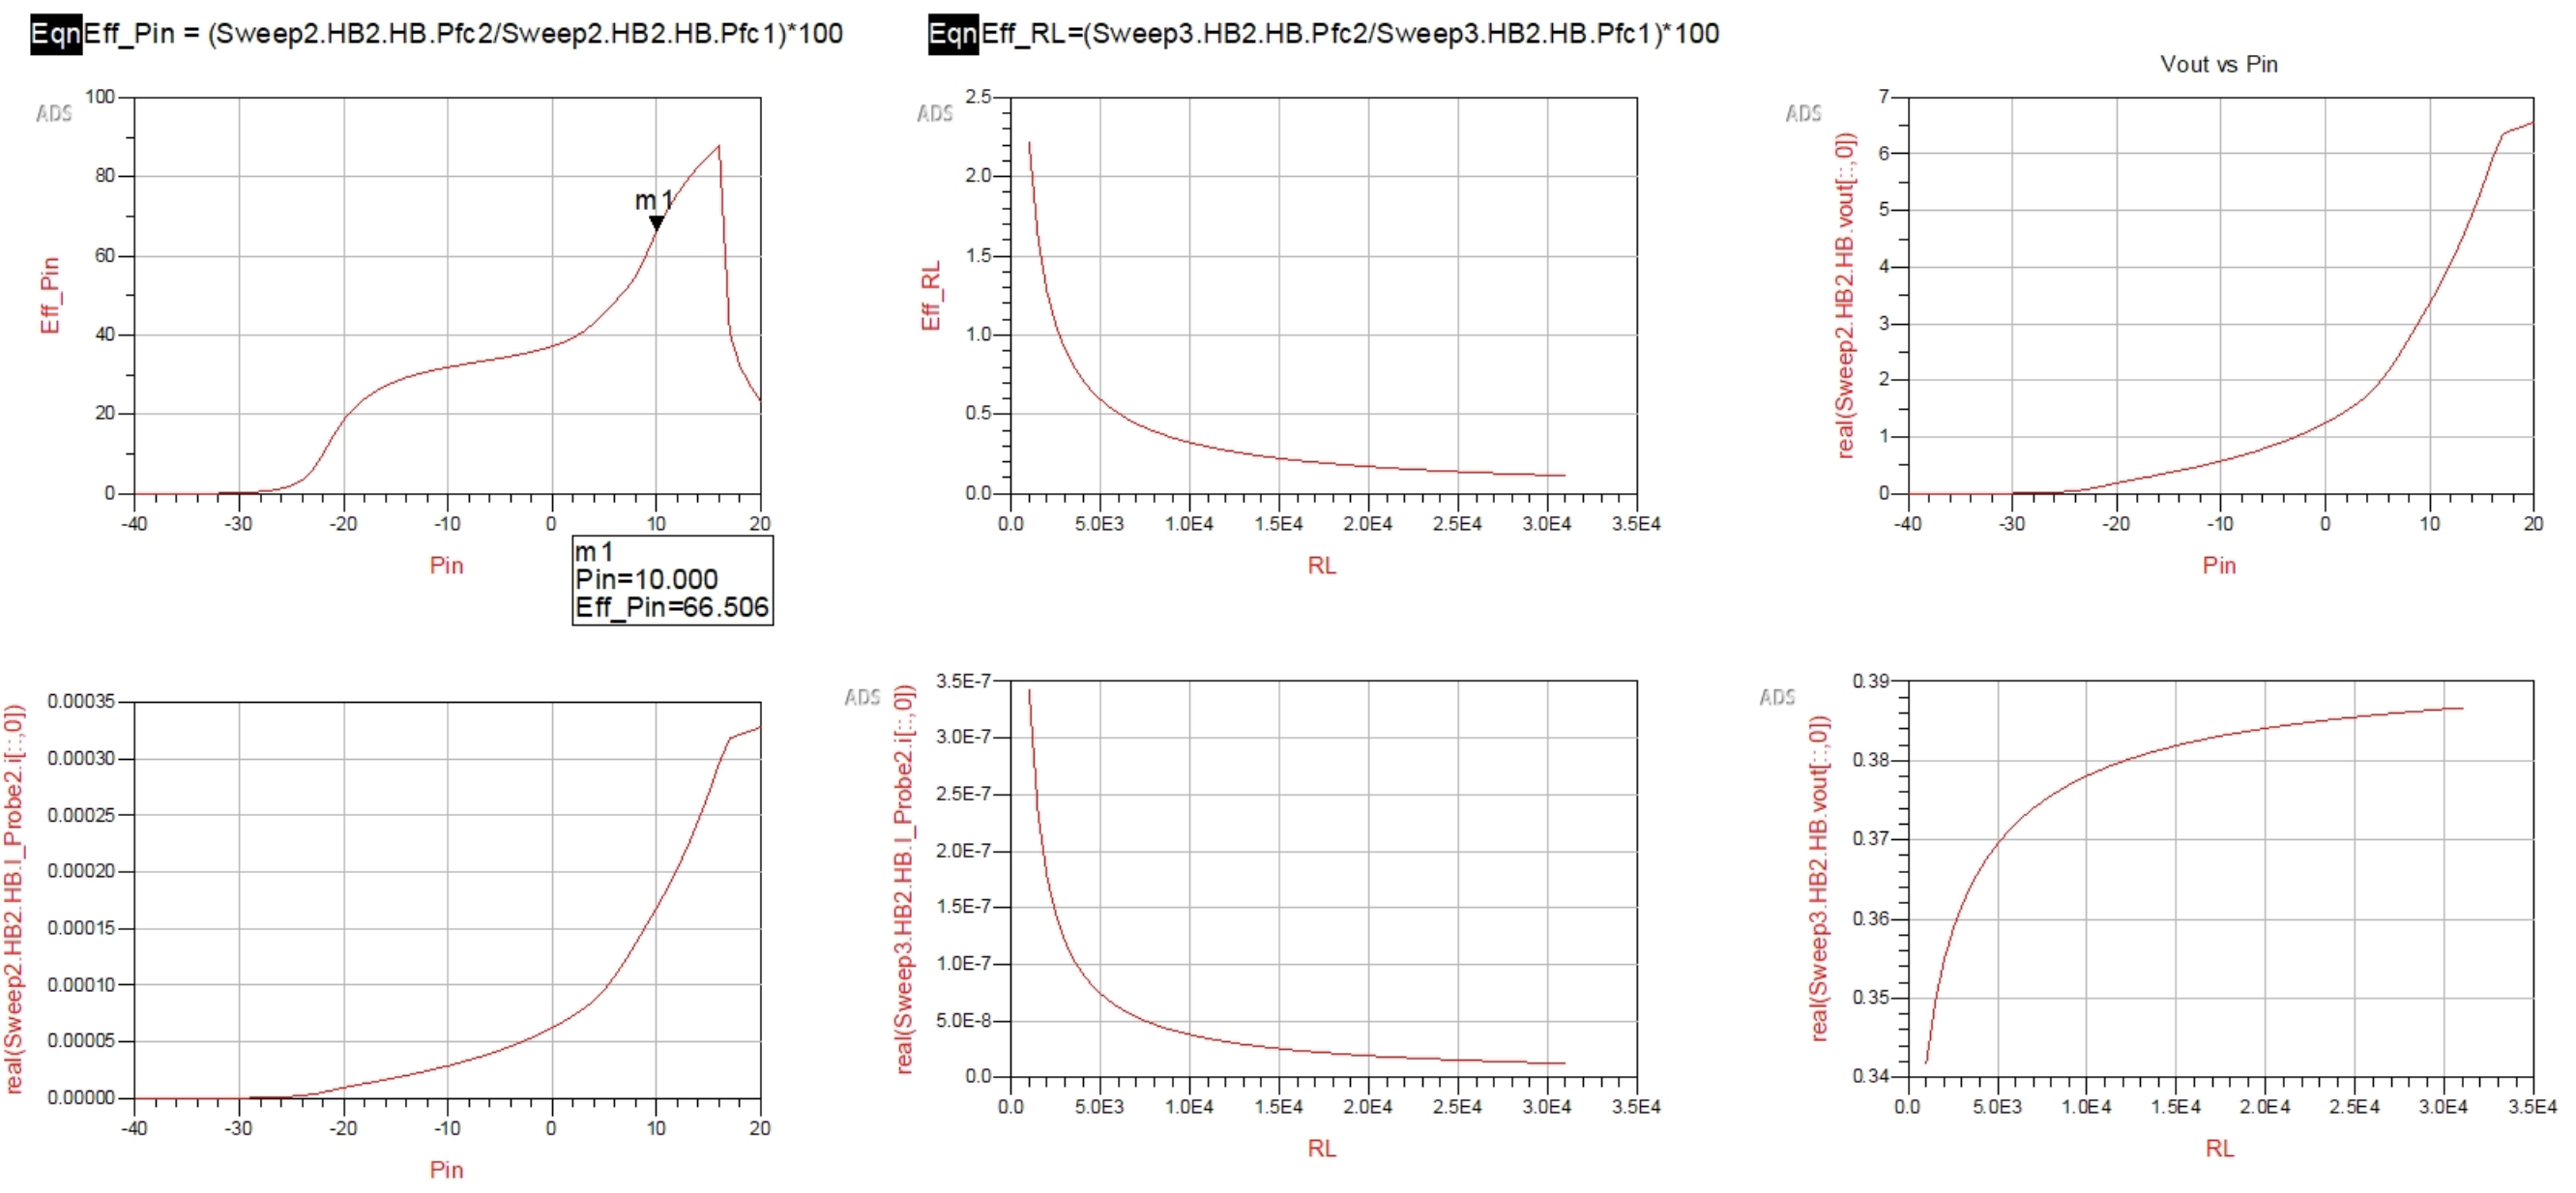
\includegraphics[width=\linewidth]{images/final_perf_2d_LC.png}
    \caption{Performance dashboard (Efficiency $\eta$, $V_\mathrm{out}$
             and $I_\mathrm{out}$) for the 2-Diode topology with hybrid
             LC + microstrip matching
             ($f = \SI{2.2}{\giga\hertz}$, $R_L = \SI{10}{\kilo\ohm}$).}
    \label{fig:final_perf_2d_LC}
\end{figure}

The hybrid LC + microstrip matching circuit achieves an efficiency of
\textbf{66.51\%} at $P_\mathrm{in} = \SI{10}{\text{dBm}}$ (Marker m1),
with an output voltage of approximately \textbf{\SI{3.8}{\volt}} at
the same power level.

Analysis of the six graphs of the hybrid LC + microstrip dashboard:
\begin{itemize}
    \item \textbf{Efficiency vs.\ $P_\mathrm{in}$:}
    The efficiency reaches an impressive \textbf{66.51\%} at our target
    $P_\mathrm{in} = \SI{10}{\text{dBm}}$ (Marker m1), and continues
    to rise above 80\% beyond \SI{10}{\text{dBm}}.
    However, this result relies entirely on ideal lumped component
    models that do not capture SMD package parasitics, component
    tolerances, or soldering variability at \SI{2.2}{\giga\hertz}.

    \item \textbf{Efficiency vs.\ $R_L$:}
    Evaluated at a constant low input power, the efficiency peaks at
    very low resistance values and drops as $R_L$ increases,
    confirming the necessity of choosing the exact right load for
    maximum power transfer.

    \item \textbf{$V_\mathrm{out}$ vs.\ $P_\mathrm{in}$:}
    The output voltage shows a steep exponential rise as the diodes
    overcome their forward voltage drop, reaching approximately
    \textbf{\SI{3.8}{\volt}} at $P_\mathrm{in} = \SI{10}{\text{dBm}}$.

    \item \textbf{$I_\mathrm{out}$ vs.\ $P_\mathrm{in}$:}
    Following Ohm's law ($I = V/R$), the output current mirrors the
    voltage curve, delivering approximately
    \textbf{\SI{0.33}{\milli\ampere}} into the \SI{10}{\kilo\ohm} load
    at $P_\mathrm{in} = \SI{10}{\text{dBm}}$.

    \item \textbf{$V_\mathrm{out}$ and $I_\mathrm{out}$ vs.\ $R_L$:}
    When swept at a constant low input power
    ($P_\mathrm{in} = -\SI{20}{\text{dBm}}$), as the load resistance
    increases, the output voltage saturates to an open-circuit
    maximum of approximately \textbf{\SI{0.39}{\volt}}, while the
    delivered current approaches zero from an initial
    value of more or less \SI{350}{\nano\ampere} at
    $R_L = \SI{1}{\kilo\ohm}$.
\end{itemize}

% --- Pure Microstrip ---
\paragraph{Pure Microstrip Matching Circuit}

Here is the schematic of the pure microstrip matching circuit:

\begin{figure}[H]
    \centering
    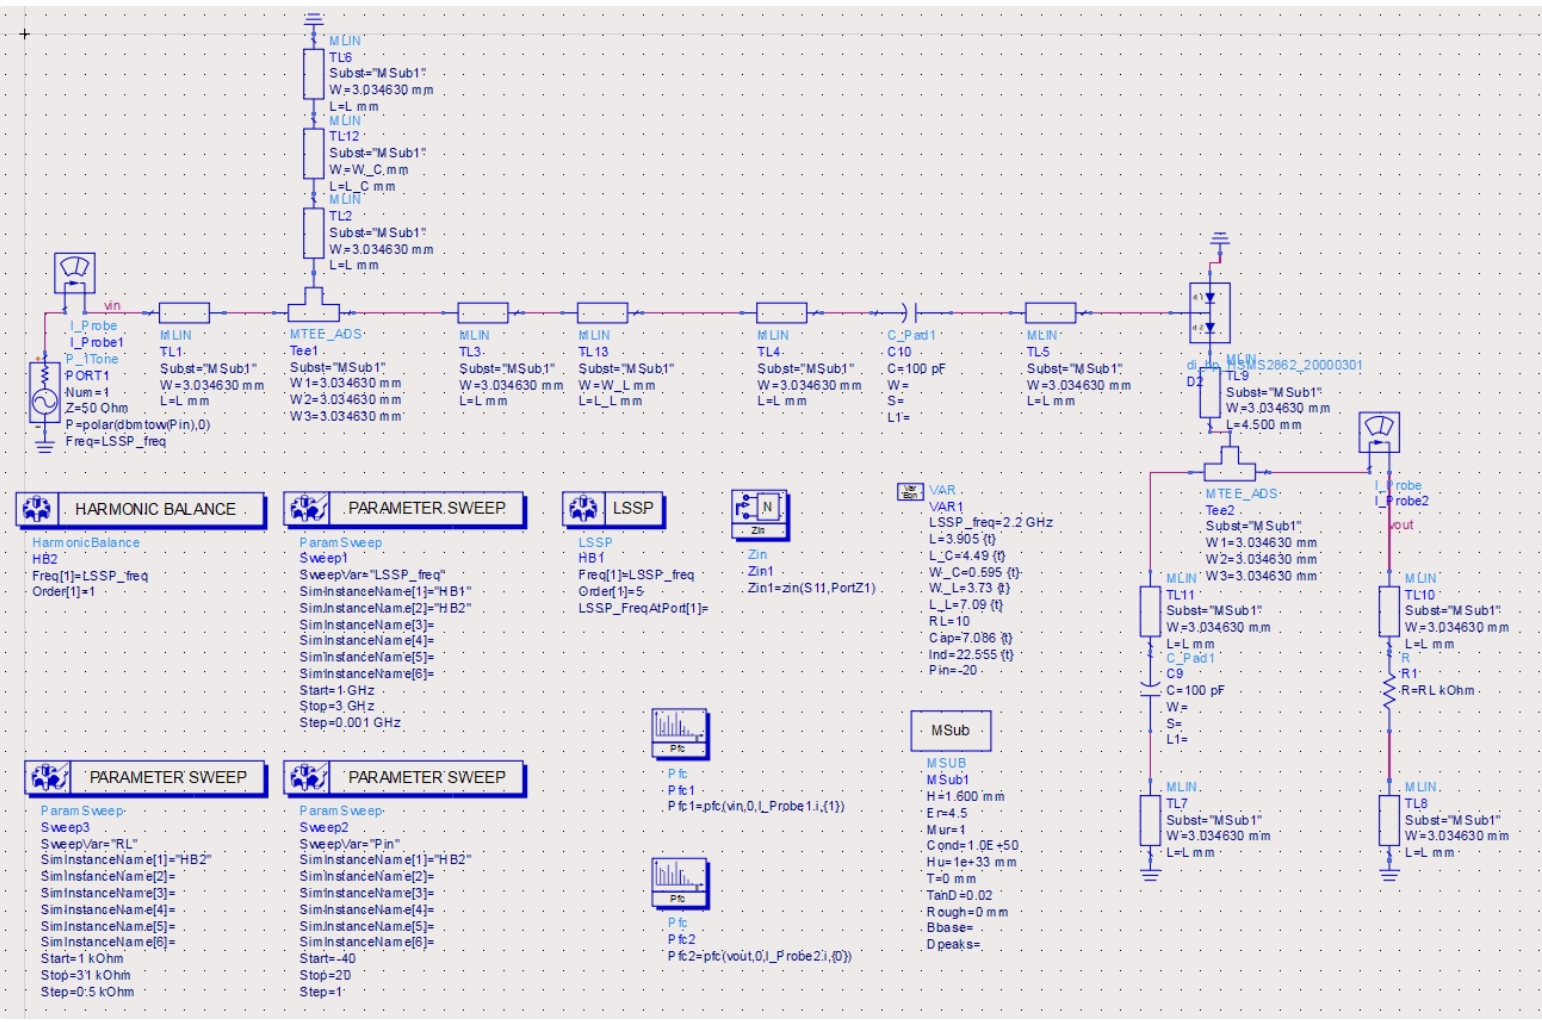
\includegraphics[width=\linewidth]{images/sch_2d_comp_ms.png}
    \caption{Harmonic Balance simulation schematic for the 2-Diode
             topology with pure microstrip matching
             ($f = \SI{2.2}{\giga\hertz}$, $R_L = \SI{10}{\kilo\ohm}$).}
    \label{fig:sch_2d_pure_ms}
\end{figure}

This topology eliminates all the SMD components from the matching
network, replacing them entirely with distributed microstrip
line segments as explained before. This approach reduces assembly
complexity, eliminates SMD parasitic effects, and is directly
transferable from the ADS layout to PCB Gerber files.

And the performance results dashboard:

\begin{figure}[H]
    \centering
    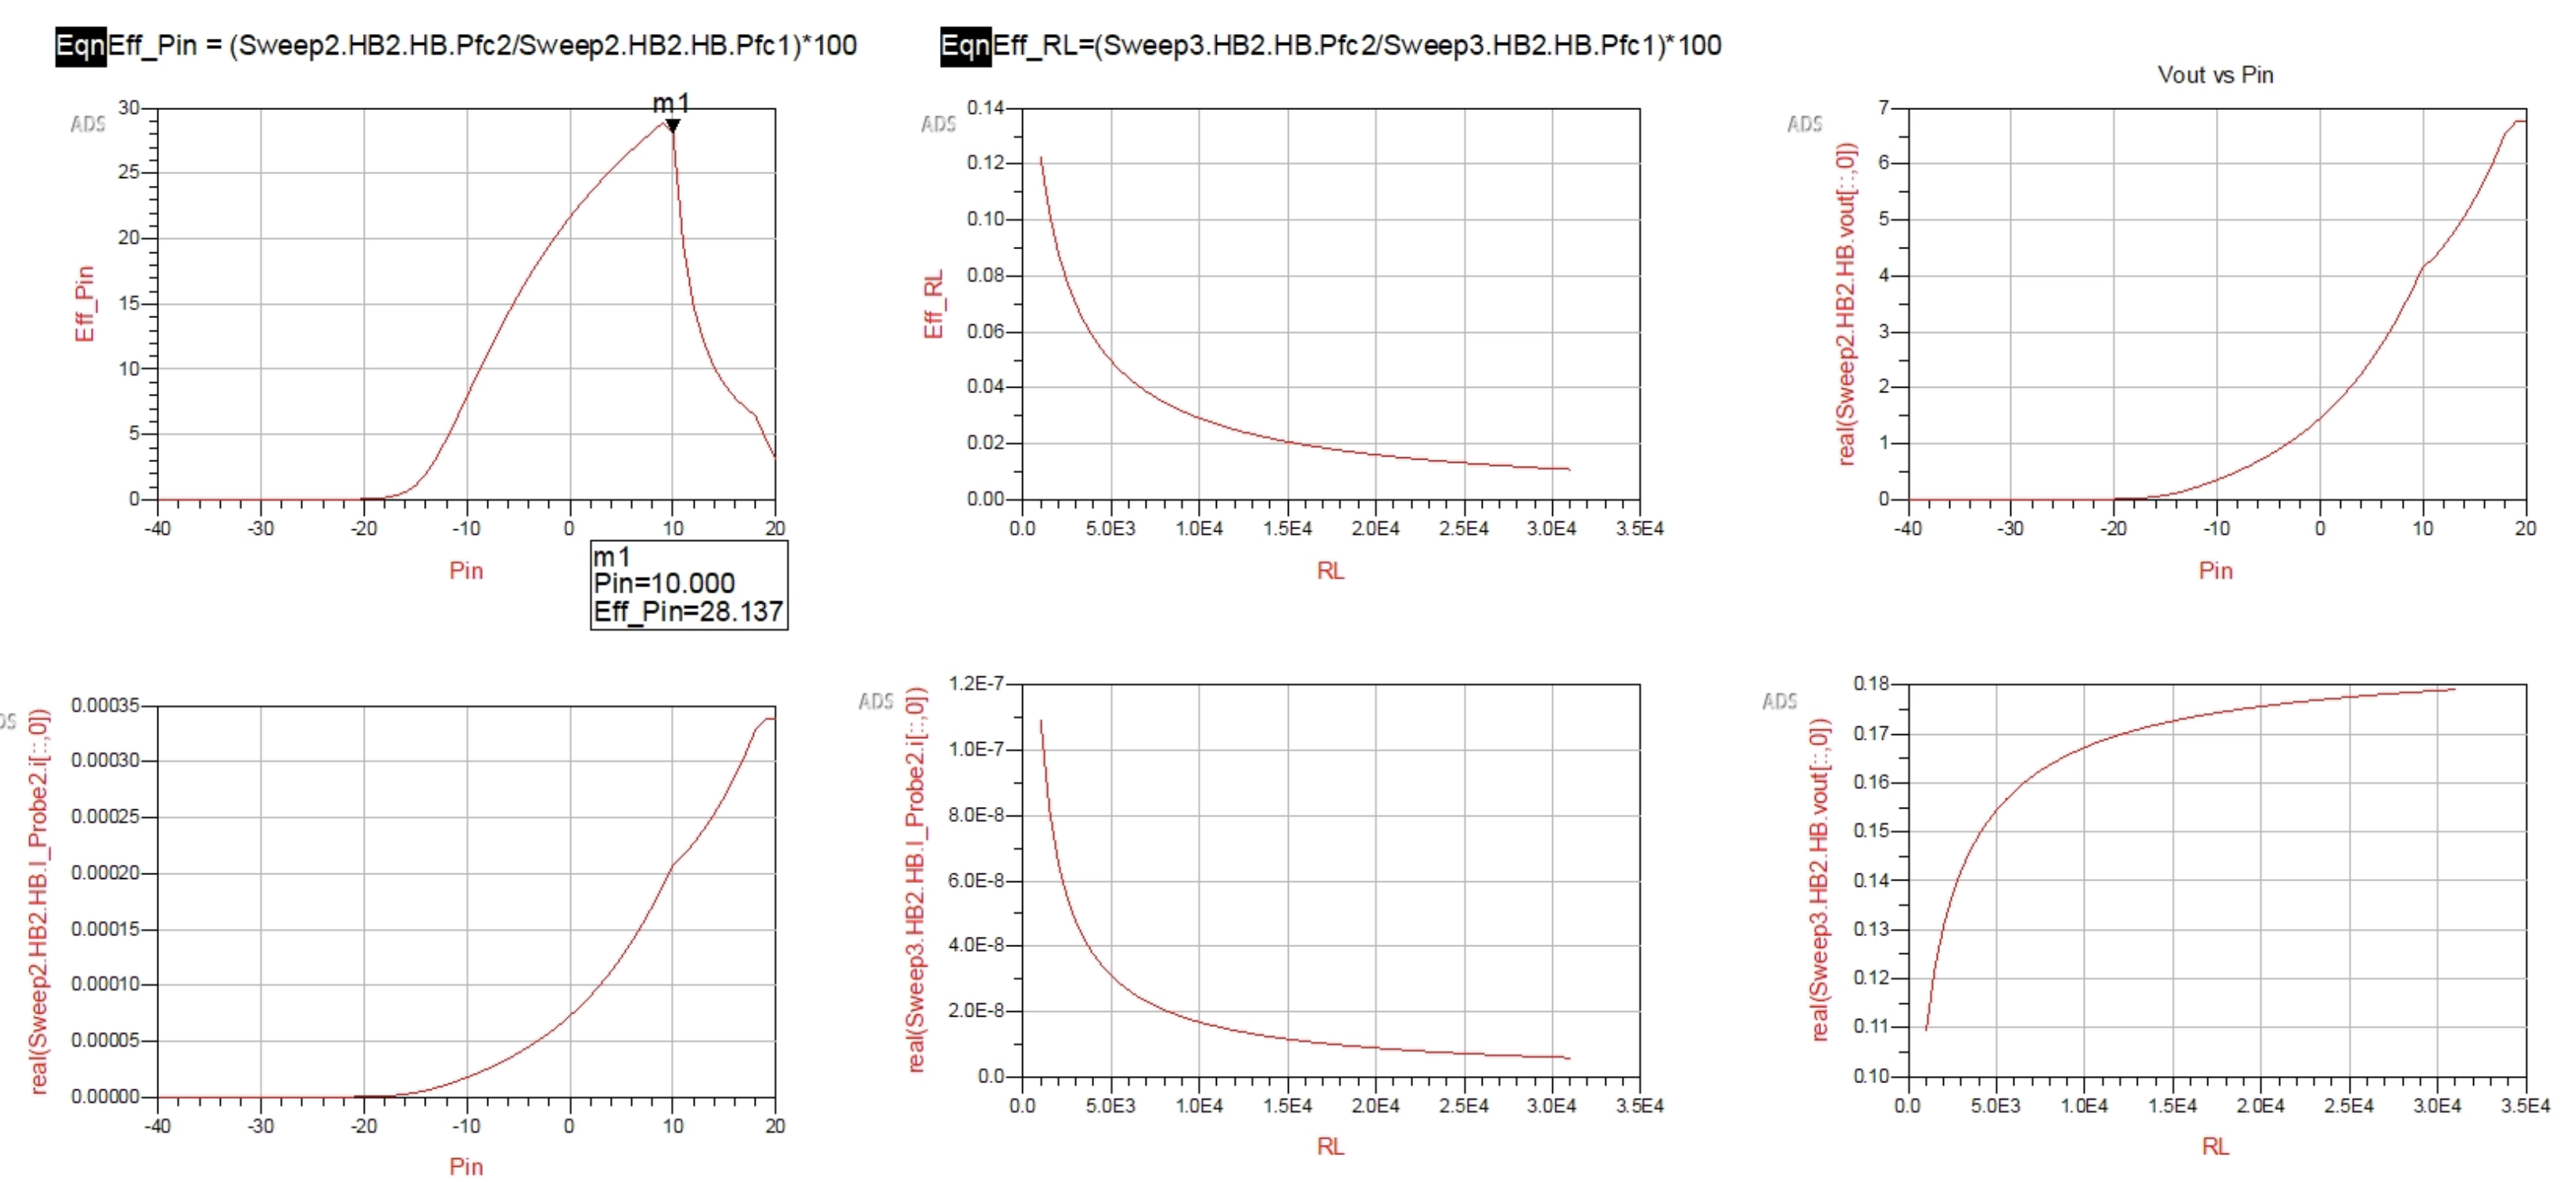
\includegraphics[width=\linewidth]{images/perf_2d_pure_ms.png}
    \caption{Performance dashboard (Efficiency $\eta$, $V_\mathrm{out}$
             and $I_\mathrm{out}$) for the 2-Diode topology with pure
             microstrip matching
             ($f = \SI{2.2}{\giga\hertz}$, $R_L = \SI{10}{\kilo\ohm}$).}
    \label{fig:perf_2d_pure_ms}
\end{figure}

The pure microstrip matching circuit achieves an efficiency of
\textbf{28.14\%} at $P_\mathrm{in} = \SI{10}{\text{dBm}}$ (Marker m1),
with an output voltage of approximately \textbf{\SI{3.2}{\volt}} at
the same power level.

Analysis of the six graphs of the pure microstrip dashboard:
\begin{itemize}
    \item \textbf{Efficiency vs.\ $P_\mathrm{in}$:}
    The efficiency is at \textbf{28.14\%} at our target
    $P_\mathrm{in} = \SI{10}{\text{dBm}}$ (Marker m1).
    It is lower than the ideal LC simulation (66.51\%), but this value
    is due to the actual dielectric and radiation losses
    of the microstrip lines.

    \item \textbf{Efficiency vs.\ $R_L$:}
    Evaluated at low input power, the efficiency peaks at very low
    resistance values (approximately 0.12\% at
    $R_L = \SI{1}{\kilo\ohm}$) and gradually drops as $R_L$ increases.
    This confirms that the circuit must be carefully matched to its
    final application for maximum power transfer.

    \item \textbf{$V_\mathrm{out}$ vs.\ $P_\mathrm{in}$:}
    The output voltage shows a steep rise as the diodes
    overcome their forward voltage drop, reaching approximately
    \textbf{\SI{3.2}{\volt}} at $P_\mathrm{in} = \SI{10}{\text{dBm}}$
    and \textbf{\SI{6.5}{\volt}} at $+\SI{20}{\text{dBm}}$.

    \item \textbf{$I_\mathrm{out}$ vs.\ $P_\mathrm{in}$:}
    Following Ohm's law, the output current follows the voltage curve,
    delivering approximately \textbf{\SI{0.17}{\milli\ampere}} into the
    \SI{10}{\kilo\ohm} load at $P_\mathrm{in} = \SI{10}{\text{dBm}}$.

    \item \textbf{$V_\mathrm{out}$ and $I_\mathrm{out}$ vs.\ $R_L$:}
    Evaluated at a constant low input power
    ($P_\mathrm{in} = -\SI{20}{\text{dBm}}$), as the load resistance
    increases, the output voltage saturates towards an open-circuit
    maximum of approximately \textbf{\SI{0.18}{\volt}}, while the
    delivered current approaches zero.
\end{itemize}

% --- Comparison ---
\subsubsection{Comparative Analysis and Topology Selection}

Table~\ref{tab:2d_comparison} summarizes the key performance metrics
of both matching topologies at $P_\mathrm{in} = \SI{10}{\text{dBm}}$
and $R_L = \SI{10}{\kilo\ohm}$.

\begin{table}[H]
    \centering
    \caption{Performance comparison of the two matching topologies
             for the 2-Diode voltage doubler at
             $P_\mathrm{in} = \SI{10}{\text{dBm}}$,
             $R_L = \SI{10}{\kilo\ohm}$, $f = \SI{2.2}{\giga\hertz}$.}
    \label{tab:2d_comparison}
    \begin{tabular}{lcc}
        \toprule
        \textbf{Metric} &
        \textbf{Hybrid LC + MS} &
        \textbf{Pure Microstrip} \\
        \midrule
        Simulated $\eta$ (\%)        & 66.51               & \textbf{28.14} \\
        Realistic $\eta$ (estimated) & LESS THAN 66.51         & \textbf{$\sim$28} \\
        $V_\mathrm{out}$ at 10\,dBm  & \SI{3.8}{\volt}     & \textbf{\SI{3.2}{\volt}} \\
        $I_\mathrm{out}$ at 10\,dBm  & \SI{330}{\micro\ampere} &
                                       \textbf{\SI{170}{\micro\ampere}} \\
        $P_\mathrm{DC}$ at 10\,dBm  & \SI{1.25}{\milli\watt} &
                                       \textbf{\SI{544}{\micro\watt}} \\
        Component count              & High                & \textbf{None} \\
        Assembly complexity          & High                & \textbf{Low} \\
        Sensitivity to tolerances    & High                & \textbf{Low} \\
        PCB transferability          & Moderate            & \textbf{Direct} \\
        \bottomrule
    \end{tabular}
\end{table}

Even if the LC topology achieves a better simulated
efficiency and output voltage, these results rely on ideal component
models that do not account for SMD package parasitics, component
tolerances, and manual soldering variability at \SI{2.2}{\giga\hertz}.
In practice, the performance gap between the two topologies would be
significantly reduced once real component non-idealities are considered.

\textbf{Conclusion:} The \textbf{pure microstrip topology} is the
preferred design for physical implementation. It delivers a fully
distributed, component-free matching network that is inherently robust
to manufacturing variability, easier to fabricate, and directly
transferable from the ADS layout to the PCB Gerber files without any
additional tuning. At $P_\mathrm{in} = \SI{10}{\text{dBm}}$, it
provides $V_\mathrm{out} \approx \SI{3.2}{\volt}$ and
$I_\mathrm{out} \approx \SI{0.17}{\milli\ampere}$, corresponding to
a DC output power of $P_\mathrm{DC} \approx \SI{544}{\micro\watt}$,
which comfortably exceeds the \SI{180}{\micro\watt} minimum requirement
of the STTS22H sensor. Furthermore, the output voltage of
\SI{3.2}{\volt} falls within the safe operating range of the sensor
(\SIrange{1.5}{3.6}{\volt}), confirming that the pure microstrip
two-diode topology is fully capable of powering the targeted
application at the design input power level.

